\documentclass{article}
\usepackage{tikz}
\usetikzlibrary{shapes,arrows}

\begin{document}

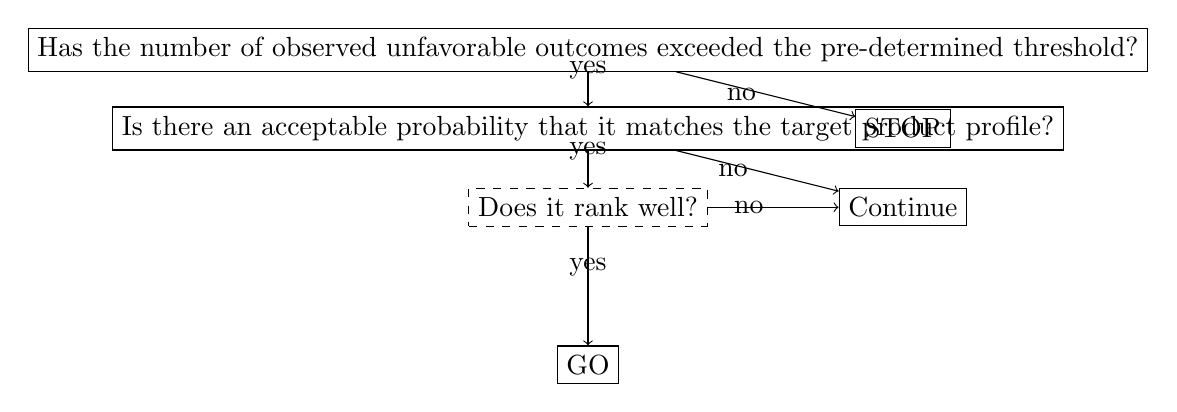
\begin{tikzpicture}[node distance=1cm]
    \node[draw] (start) {Has the number of observed unfavorable outcomes exceeded the pre-determined threshold?};
    \node[draw, below of=start] (question1) {Is there an acceptable probability that it matches the target product profile?};
    \node[draw, dashed, below of=question1] (question2) {Does it rank well?};
    \node[draw, right of=question1, xshift=3cm] (stop) {STOP};
    \node[draw, right of=question2, xshift=3cm] (continue) {Continue};
    \node[draw, below of=question2, yshift=-1cm] (go) {GO};

    \draw[->] (start) -- node[anchor=south] {yes} (question1);
    \draw[->] (start) -- node[anchor=east] {no} (stop);
    \draw[->] (question1) -- node[anchor=south] {yes} (question2);
    \draw[->] (question1) -- node[anchor=east] {no} (continue);
    \draw[->] (question2) -- node[anchor=south] {yes} (go);
    \draw[->] (question2) -- node[anchor=east] {no} (continue);
\end{tikzpicture}

\end{document}